\documentclass{sigchi}

% Use this command to override the default ACM copyright statement (e.g. for preprints). 
% Consult the conference website for the camera-ready copyright statement.


%% EXAMPLE BEGIN -- HOW TO OVERRIDE THE DEFAULT COPYRIGHT STRIP -- (July 22, 2013 - Paul Baumann)
\toappear{To appear in the iGAM4ER 2014 - Paris, France.}
%% EXAMPLE END -- HOW TO OVERRIDE THE DEFAULT COPYRIGHT STRIP -- (July 22, 2013 - Paul Baumann)


% Arabic page numbers for submission. 
% Remove this line to eliminate page numbers for the camera ready copy
% \pagenumbering{arabic}


% Load basic packages
\usepackage{balance}  % to better equalize the last page
\usepackage{graphics} % for EPS, load graphicx instead
\usepackage{times}    % comment if you want LaTeX's default font
\usepackage{url}      % llt: nicely formatted URLs
\usepackage{tabu}
\usepackage{subcaption}
\usepackage{enumitem}
\usepackage{multicol}

% llt: Define a global style for URLs, rather that the default one
\makeatletter
\def\url@leostyle{%
  \@ifundefined{selectfont}{\def\UrlFont{\sf}}{\def\UrlFont{\small\bf\ttfamily}}}
\makeatother
\urlstyle{leo}


% To make various LaTeX processors do the right thing with page size.
\def\pprw{8.5in}
\def\pprh{11in}
\special{papersize=\pprw,\pprh}
\setlength{\paperwidth}{\pprw}
\setlength{\paperheight}{\pprh}
\setlength{\pdfpagewidth}{\pprw}
\setlength{\pdfpageheight}{\pprh}

% Make sure hyperref comes last of your loaded packages, 
% to give it a fighting chance of not being over-written, 
% since its job is to redefine many LaTeX commands.
\usepackage[pdftex]{hyperref}
\hypersetup{
bookmarksnumbered,
pdfstartview={FitH},
colorlinks,
citecolor=black,
filecolor=black,
linkcolor=black,
urlcolor=black,
breaklinks=true,
}

% create a shortcut to typeset table headings
\newcommand\tabhead[1]{\small\textbf{#1}}

% path of images
\graphicspath{{./images/}}

% Shared affiliations
\def\sharedaffiliation{%
\end{tabular}
\begin{tabular}{c}}

% To keep the url in the same font of the institution address
\newcommand{\urlwofont}[1]{\urlstyle{same}\url{#1}}

% Column types for text
\newcolumntype{L}[1]{>{\raggedright\let\newline\\\arraybackslash\hspace{0pt}}m{#1}}
\newcolumntype{C}[1]{>{\centering\let\newline\\\arraybackslash\hspace{0pt}}m{#1}}
\newcolumntype{R}[1]{>{\raggedleft\let\newline\\\arraybackslash\hspace{0pt}}m{#1}}

\newcommand{\refsectitle}[1]{\ref{#1}~(\nameref{#1})}

% End of preamble. Here it comes the document.
\begin{document}

% Define the name of the game
\newcommand{\gamename}{Ice Cream Factory}
\title{\gamename: a digital game to foster learning computer programming skills}

\numberofauthors{4}
\author{
	\alignauthor Vin\'icius Kiwi Daros\\
		\email{vkdaros@ime.usp.br}
%
	\alignauthor Luiz Carlos Vieira\\
		\email{lvieira@ime.usp.br}
%
	\alignauthor Adalberto Bosco C. Pereira\\
		\email{bosco@ime.usp.br}
%
	\alignauthor Fl\'avio Soares C. da Silva\\
		\email{fcs@ime.usp.br}
%
	\sharedaffiliation  
		\affaddr{Laboratory of Interactivity and Digital Entertainment Technology}\\
		\affaddr{Department of Computer Science, Institute of Mathematics and Statistics}\\
		\affaddr{University of S\~ao Paulo -- Rua do Mat\~ao, 1010, CEP 05508-090, S\~ao Paulo, SP, Brazil}\\
		\affaddr{\urlwofont{http://www.ime.usp.br/~lidet}}
}
\maketitle

\begin{abstract}
Yada yada yada
\end{abstract}

\keywords{
	games; education; computer programming; logical thinking; Brazilian fauna
}

\category{K.3.1.}{Computer Uses in Education}{Computer-assisted instruction (CAI)}
\category{K.8.0.}{Personal Computing}{Games}

\section{Introduction}

	\renewcommand{\gamename}{\textit{\textbf{Ice Cream Factory}}}
	
	In all developed countries, primary school children have at least one class a week when they use a computer \cite{Istrate2010}, but so far computers have been mostly employed to aid in other disciplines and as a productivity tool. So that it has been argued that young people should be educated not only in the application and use of technology, but also in \textit{how it works} and what are its \textit{fundamental principles}. A report prepared for the UK Computing Research Committee \cite{Jones2009} particularly mentions the fact that UK students are now becoming disenchanted with the computer aided learning because they arrive at school with a much richer background in ICT (Information and Communication Technology) than that offered at their schools. The report also advocates that if on one hand learning how to use computers can be seen as similar to learning how to read, on the other hand learning how to program computers is similar to learning how to write. They are both skills that everyone should have, even though only a minority will become professionals (writers or computer programmers).
	
	Despite good arguments both in favor and against the use of computers by children \cite{Istrate2010,Setzer2001}, the study of computer programming at primary and secondary school is increasingly being acknowledged as equally important as other disciplines such as math or science. The main reason is that the skills required for programming computers are definitely valuable for education \cite{Kahn1999}, since they involve procedural thinking, problem solving through trial and error, creativity, thinking about thinking, and the analysis and exploration of data:
	
	\begin{quotation}
		\noindent
		\emph{In programming, it is important to provide models for the students to emulate. Programming has elements of good design that make it a great learning experience: the iterative process towards a solution, the ultimate goal that has many paths and choices on the way, and the mistakes that provide feedback and experience.}
	\end{quotation}
	
	The experience the authors of this paper have had in teaching basic computer programming at the graduation course in Administration of the University of S\~ao Paulo corroborates that even when employing tools that the students are required to use in their daily routines and accustomed with -- such as the Microsoft Office Excel\footnote{\url{http://office.microsoft.com/excel}} with its Visual Basic for Applications programming language, the task of learning how to use control structures in planning and solving problems by iterative execution is still perceived as very boring even for older students.
	
	As consequence, the LIDET (Laboratory of Interactivity and Digital Entertainment Technology) team at the University of S\~ao Paulo has been working on the development of a digital game called \gamename, which will have educational intentions mainly related to the development of skills necessary for programming computational tasks. This text is being submitted as the partial requirement for registering in the iGAM4ER 2014 contest. The next sections will describe existing similar games and the game under construction in more details.

\section{Similar Existing Games}

\section{The Construction of \gamename}

\section{Educational Aspects Addressed}

\section{Concept Art}

	Here are some sketches of the concept art for the game.
	\begin{center}
		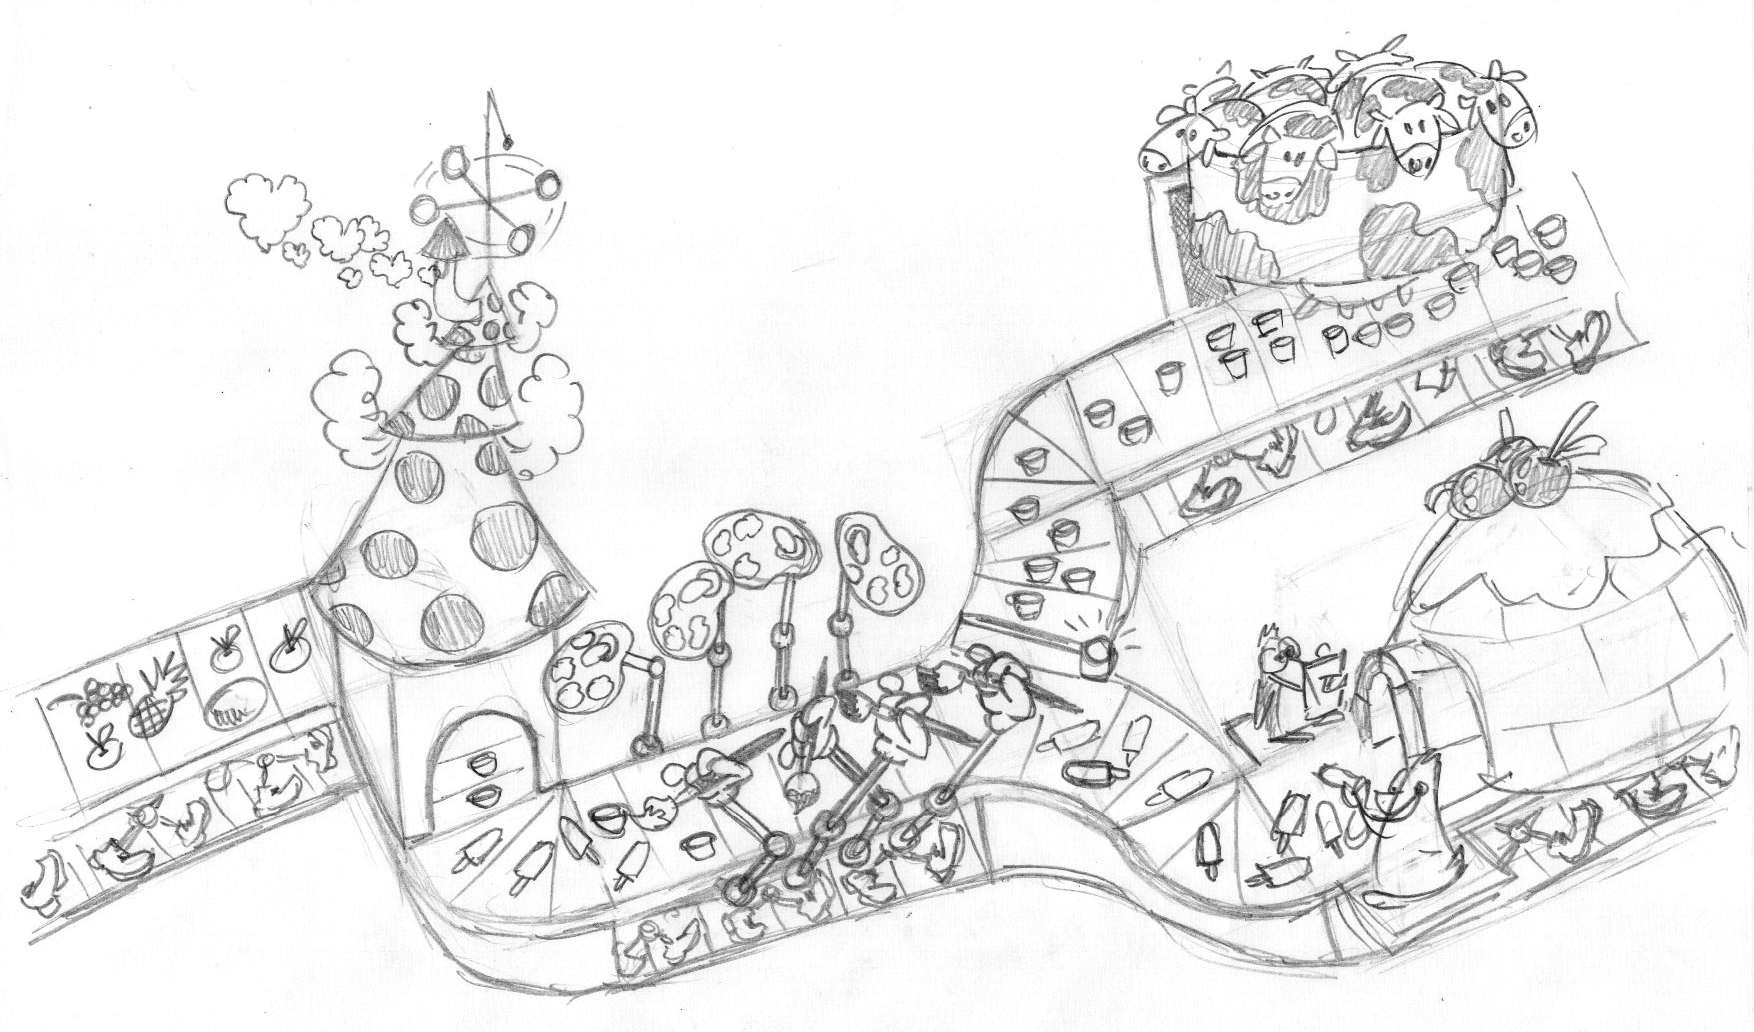
\includegraphics[width=0.9\columnwidth]{01}
		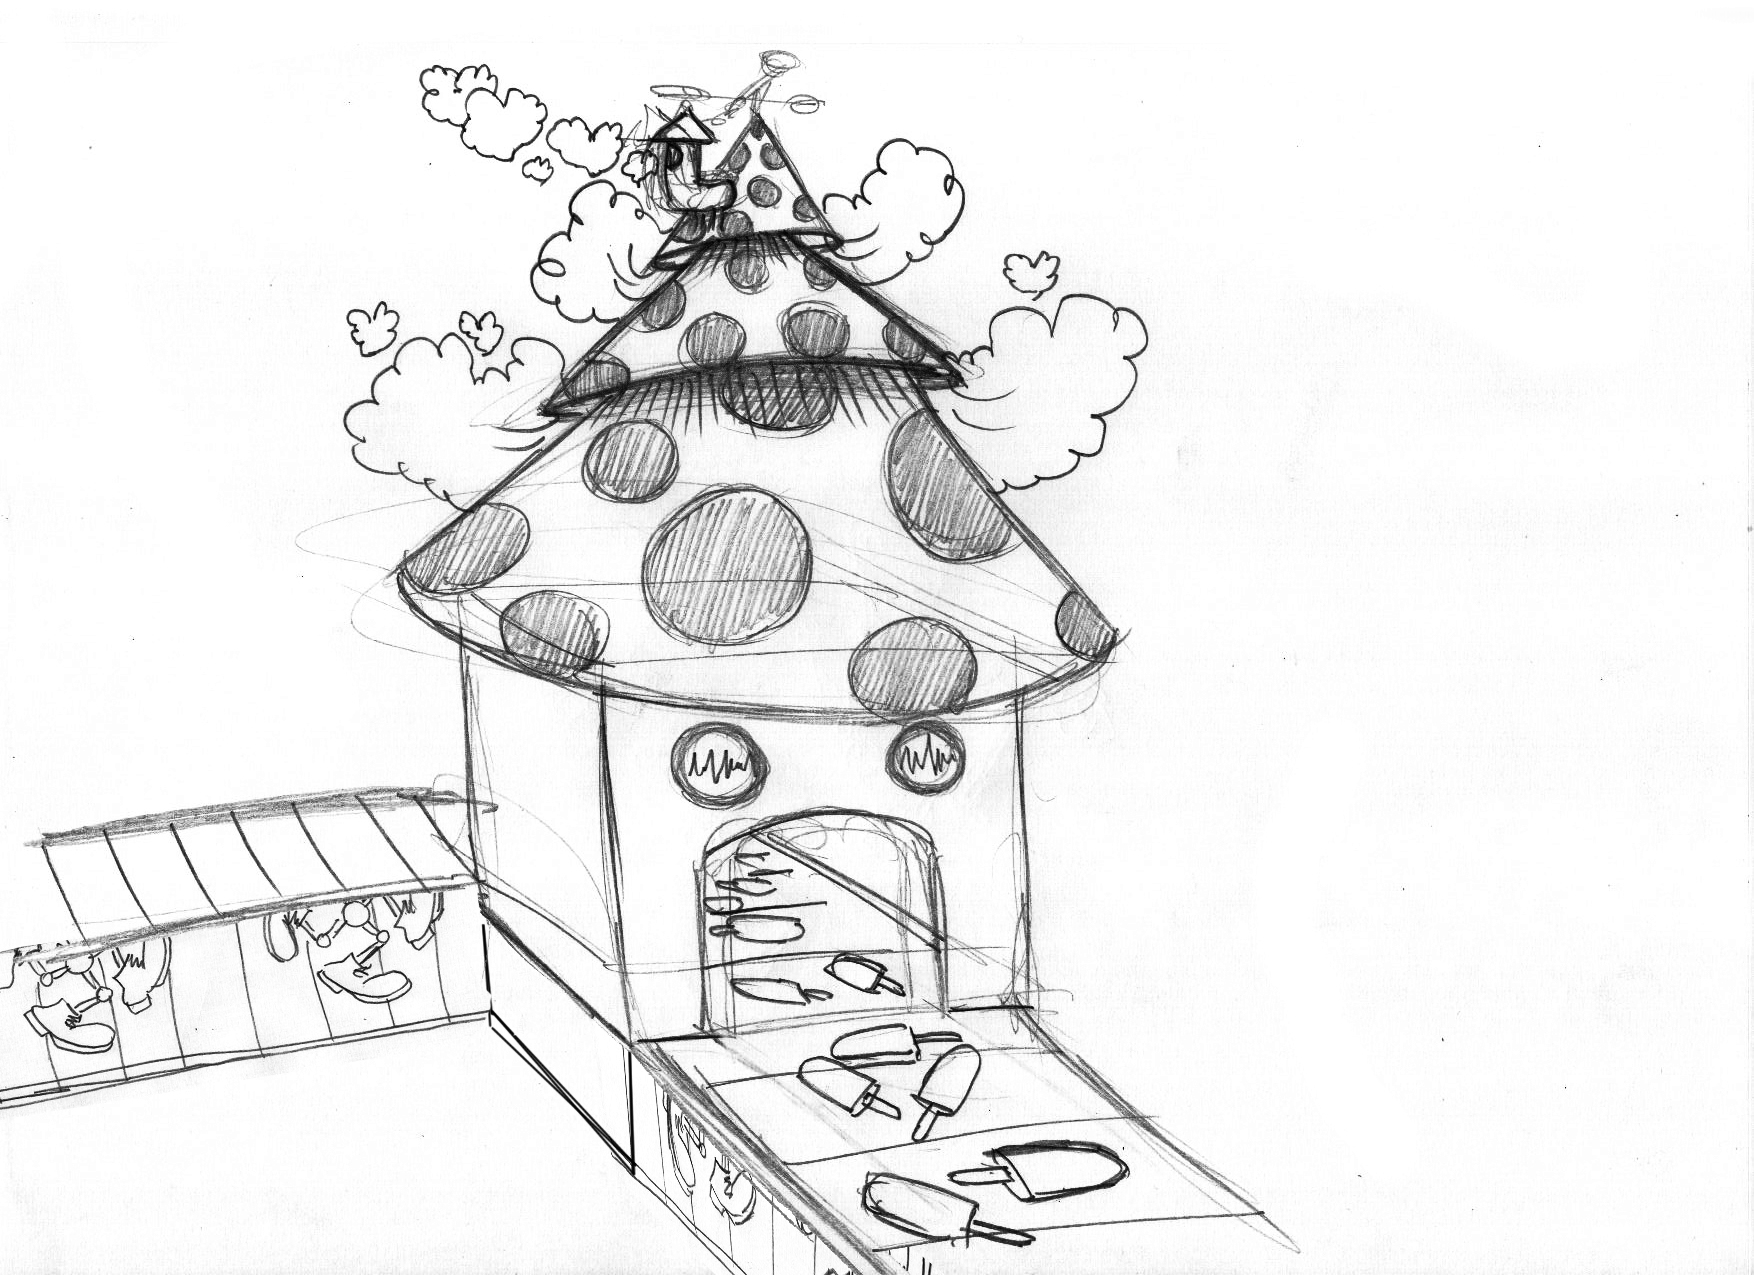
\includegraphics[width=0.9\columnwidth]{02}
		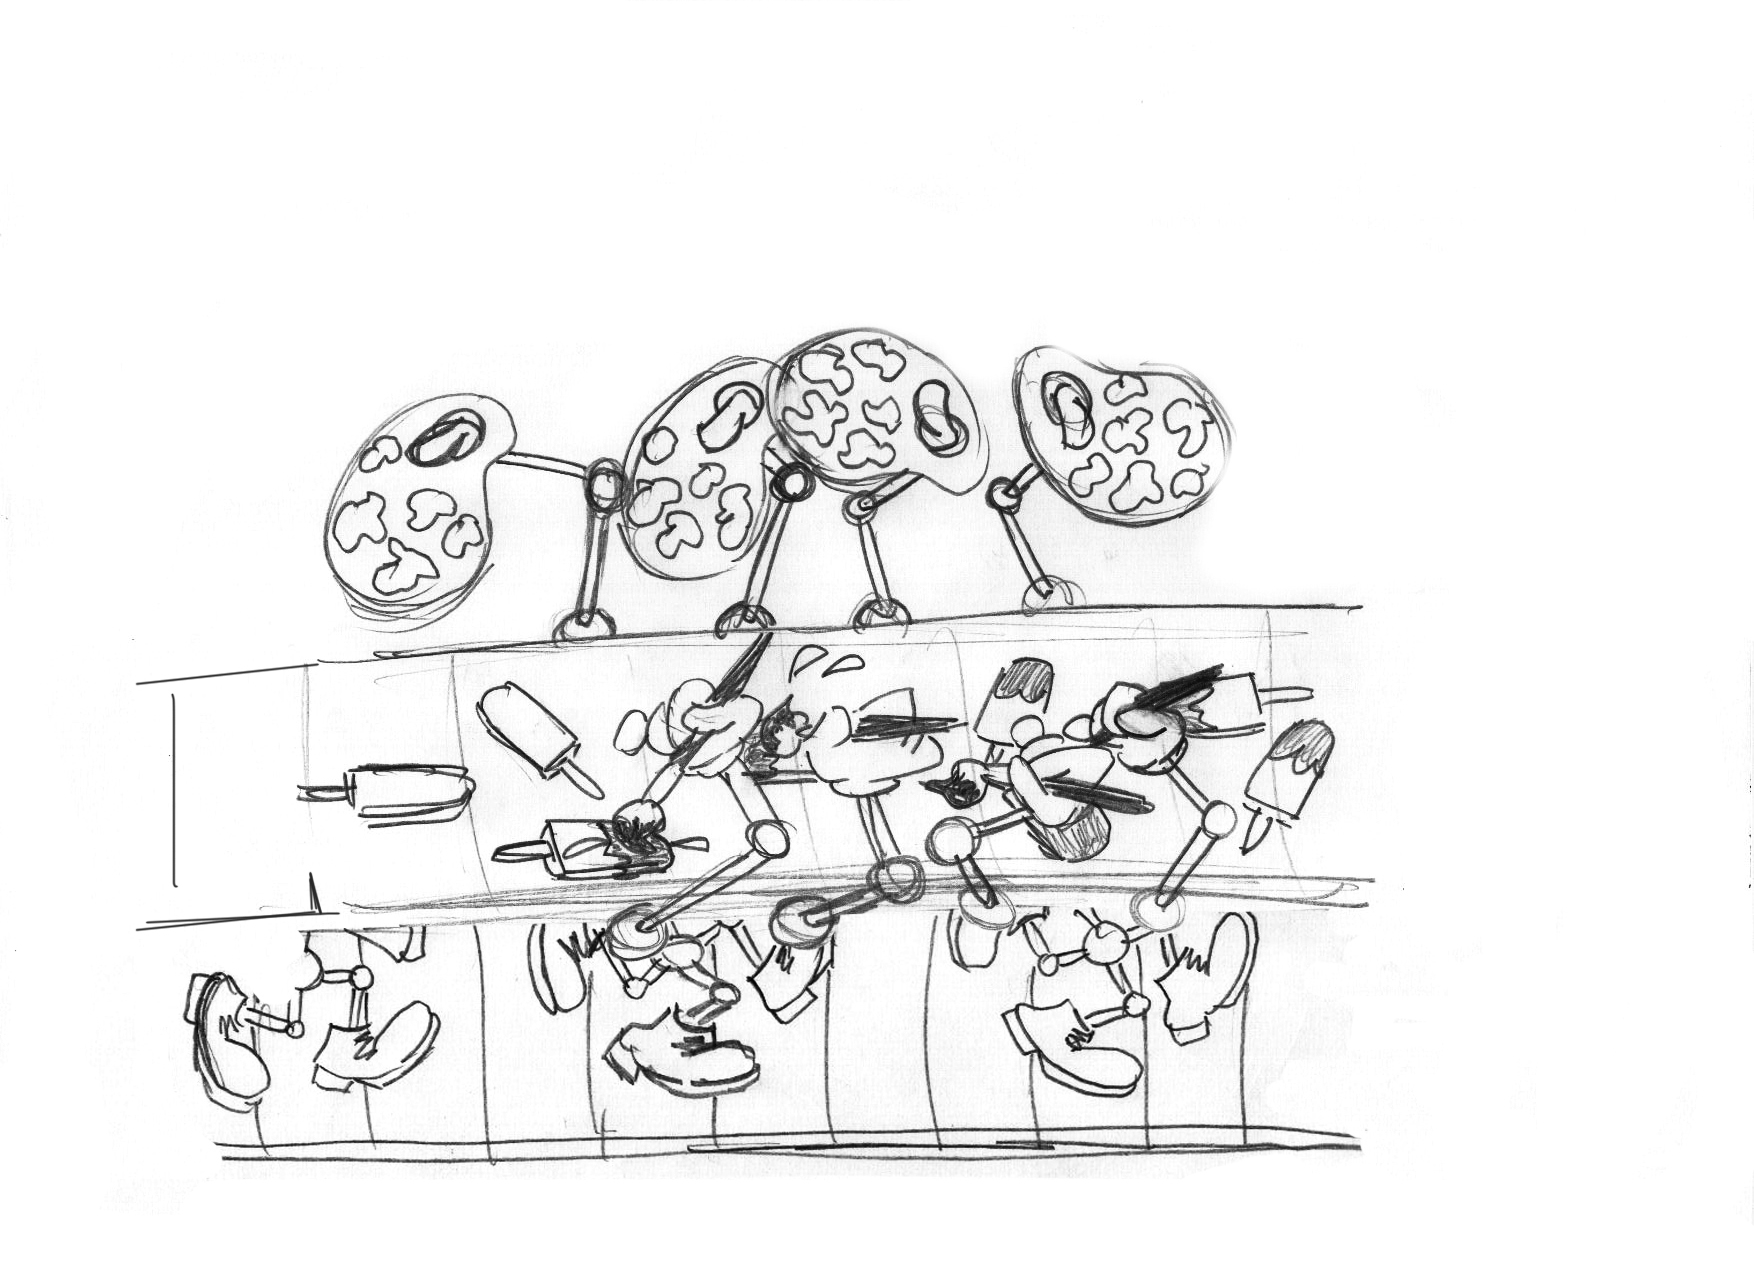
\includegraphics[width=0.9\columnwidth]{03}
		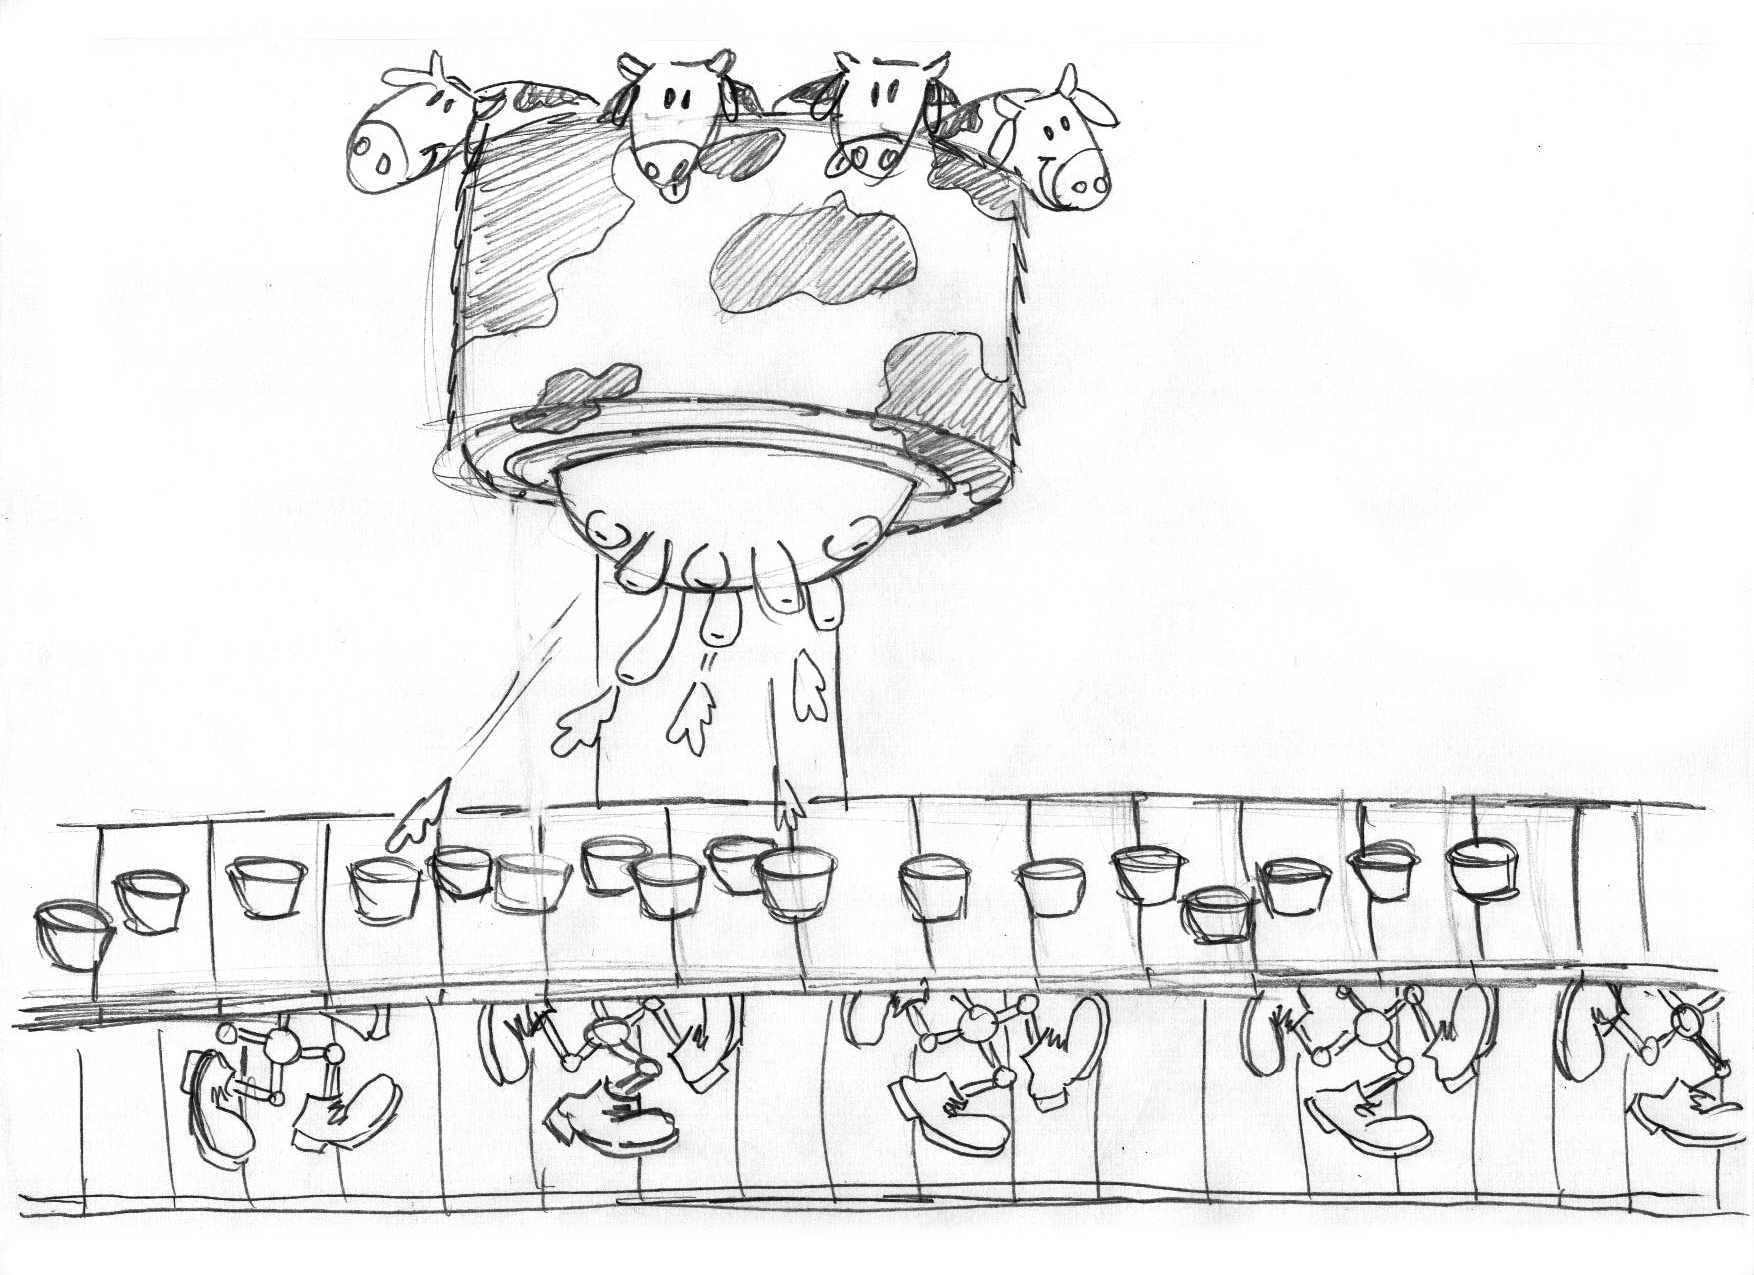
\includegraphics[width=0.9\columnwidth]{04}
		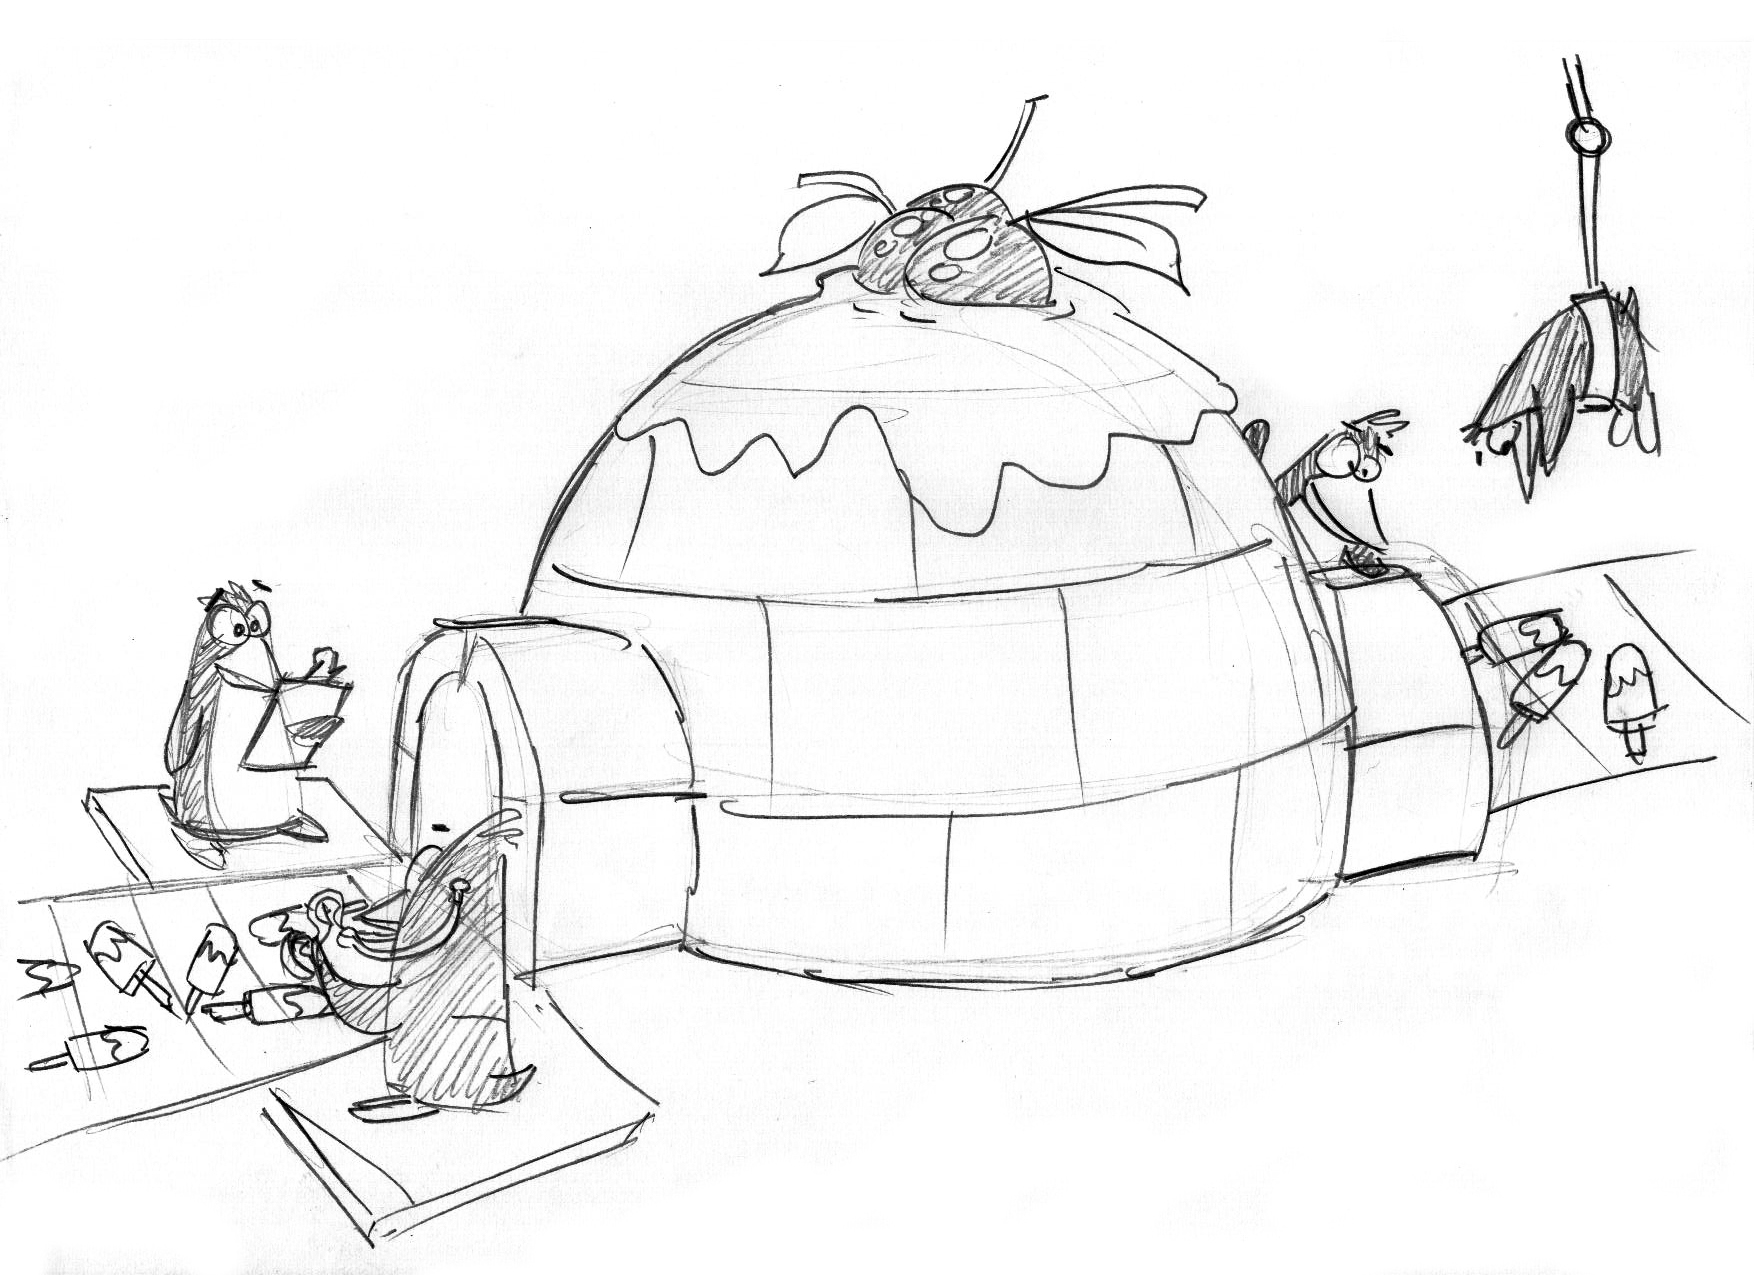
\includegraphics[width=0.9\columnwidth]{05}
		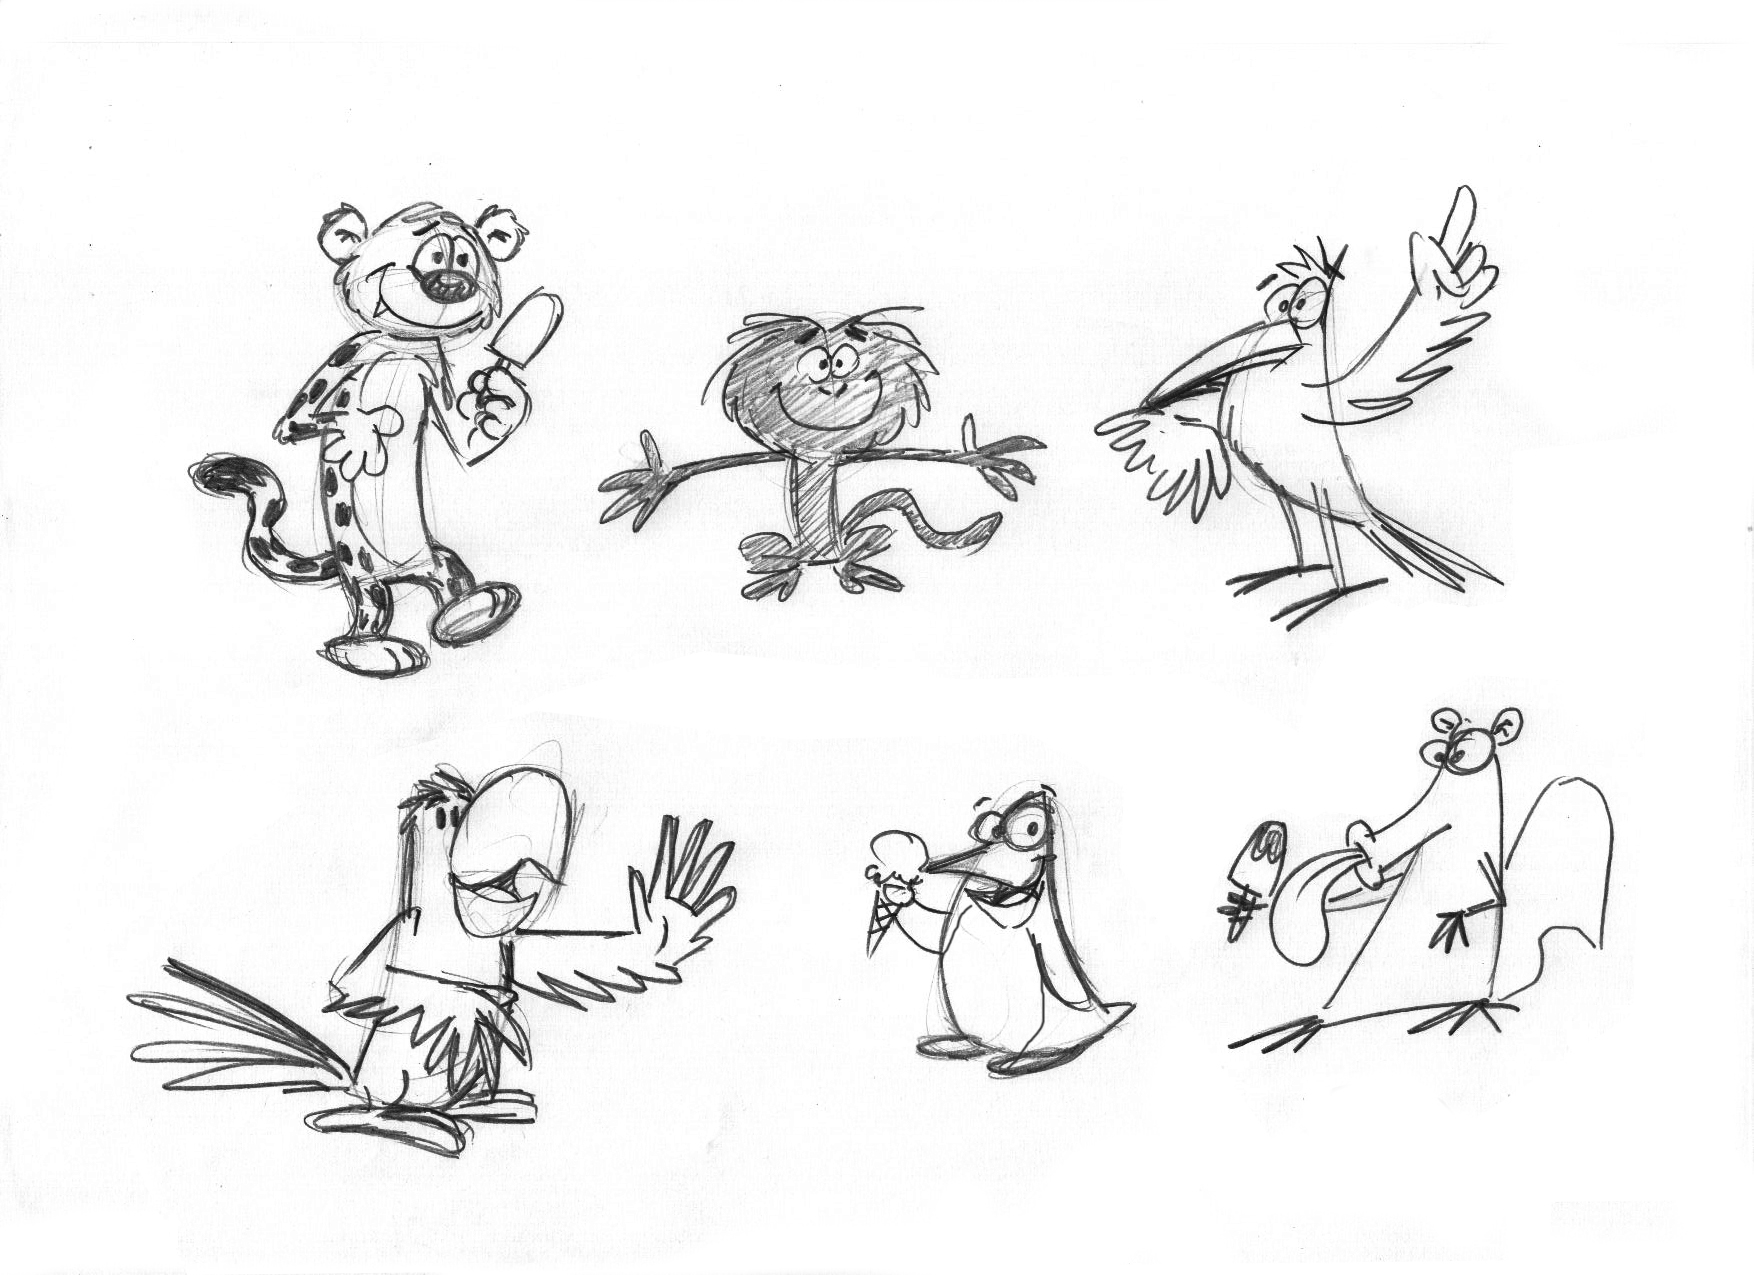
\includegraphics[width=0.9\columnwidth]{06}
	\end{center}

\section{Acknowledgments}

	The authors would like to thank CAPES (\textit{Coordena\c{c}\~ao de Aperfei\c{c}oamento de Pessoal de N\'ivel Superior}) and CRI (Center for Research and Interdisciplinarity) for the financial support. The authors also thank the artist Danilo G. Rios for the concept art.

% Balancing columns in a ref list is a bit of a pain because you
% either use a hack like flushend or balance, or manually insert
% a column break.  http://www.tex.ac.uk/cgi-bin/texfaq2html?label=balance
% multicols doesn't work because we're already in two-column mode,
% and flushend isn't awesome, so I choose balance.  See this
% for more info: http://cs.brown.edu/system/software/latex/doc/balance.pdf
%
% Note that in a perfect world balance wants to be in the first
% column of the last page.
%
% If balance doesn't work for you, you can remove that and
% hard-code a column break into the bbl file right before you
% submit:
%
% http://stackoverflow.com/questions/2149854/how-to-manually-equalize-columns-
% in-an-ieee-paper-if-using-bibtex
%
% Or, just remove \balance and give up on balancing the last page.
%
\balance

\bibliographystyle{acm-sigchi}
\bibliography{igamer_bib}
\end{document}
